\documentclass[xcolor=pdftex,dvipsnames,table]{beamer}
\usetheme{Darmstadt}
\usepackage{etex}
\providecommand\thispdfpagelabel[1]{}
\usepackage[latin1]{inputenc}
\usepackage{amsmath}
\usepackage{amssymb}
\usepackage{amsthm}
\usepackage{listings}
\usepackage{graphics}
\usepackage{framed}
\usepackage{etex}
\usepackage[all]{xy}
\usepackage{xspace,listings,ulem,tikz}
\usepackage[outline]{contour}
\contourlength{1.2pt}
\usepackage[square,sort,comma,numbers]{natbib}
\setbeamertemplate{footline}[frame number]
\tikzset{
    onslide/.code args={<#1>#2}{% http://tex.stackexchange.com/a/6155/16595
        \only<#1>{\pgfkeysalso{#2}}
    },
    hideshow/.style args={<#1><#2>#3}{%
        onslide=<#1>{move to},
        onslide=<#2>{#3}
    }
}
\lstset{
         basicstyle=\footnotesize\ttfamily, % Standardschrift
         %numbers=left,               % Ort der Zeilennummern
         numberstyle=\tiny,          % Stil der Zeilennummern
         %stepnumber=2,               % Abstand zwischen den Zeilennummern
         numbersep=5pt,              % Abstand der Nummern zum Text
         tabsize=2,                  % Groesse von Tabs
         extendedchars=true,         %
         breaklines=true,            % Zeilen werden Umgebrochen
         keywordstyle=\color{red},
    		frame=b,         
 %        keywordstyle=[1]\textbf,    % Stil der Keywords
 %        keywordstyle=[2]\textbf,    %
 %        keywordstyle=[3]\textbf,    %
 %        keywordstyle=[4]\textbf,   \sqrt{\sqrt{}} %
         %stringstyle=\color{white}\ttfamily, % Farbe der String
         showspaces=false,           % Leerzeichen anzeigen ?
         showtabs=false,             % Tabs anzeigen ?
         xleftmargin=3pt,
         framexleftmargin=3pt,
         framexrightmargin=1pt,
         framexbottommargin=3pt,
         language=C++,
         %backgroundcolor=\color{lightgray},
         showstringspaces=false      % Leerzeichen in Strings anzeigen ?        
 }

 \usetikzlibrary{arrows}
 \usepackage{caption}
\DeclareCaptionFont{white}{\color{white}}
\DeclareCaptionFormat{listing}{\colorbox[cmyk]{0.43, 0.35, 0.35,0.01}{\parbox{\textwidth}{\hspace{15pt}#1#2#3}}}
\captionsetup[lstlisting]{format=listing,labelfont=white,textfont=white, singlelinecheck=false, margin=0pt, font={bf,footnotesize}}
\beamertemplatenavigationsymbolsempty
\newcommand{\N}{\ensuremath{\mathbb{N}}} 
\newcommand{\R}{\ensuremath{\mathbb{R}}} 
\newcommand{\RR}{\ensuremath{\mathbb{R}}} 
\newcommand{\C}{\ensuremath{\mathbb{C}}} 
\newcommand{\Q}{\ensuremath{\mathbb{Q}}} 
\newcommand{\Z}{\ensuremath{\mathbb{Z}}} 
\newcommand{\D}{\ensuremath{\mathbb{D}}}
\newcommand{\lb}{\mathrm{lb}}
\newcommand{\dy}{\mathrm{dy}}
\newcommand{\cc}{\texttt{C++}\xspace}
\newcommand{\bin}{\mathrm{bin}}
\newcommand{\irram}{\texttt{iRRAM}\xspace}
\newcommand{\code}[1]{\texttt{#1}}
\newcommand{\sharpp}{\ensuremath{\#\mathcal P}\xspace}
\newcommand{\sharppu}{\ensuremath{\#{\mathcal P}_1}\xspace}
\newcommand{\fp}{\ensuremath{\mathcal{FP}}\xspace}
  \newcommand{\baana}{\code{BA\_ANA}\xspace}
  \newcommand{\anarect}{\code{ANA\_RECT}\xspace}
  \newcommand{\powerseries}{\code{POWERSERIES}\xspace}
  \newcommand{\poly}{\code{POLY}\xspace}
  \newcommand{\func}{\code{FUNC}\xspace}
  \newcommand{\real}{\code{REAL}\xspace}
  \newcommand{\complex}{\code{COMPLEX}\xspace}
  \newcommand{\temp}{\textcolor{red}}
  \newcommand{\seq}{\mathbf}
\newcommand{\fpu}{\ensuremath{\mathcal{FP}_1}\xspace}
\DeclareMathOperator{\dom}{\mathrm{dom}}
\newtheorem{conjecture}{Conjecture} 
\newtheorem{representation1}{Representation 1} 
\newtheorem{representation1b}{Representation 1'} 
\newtheorem{representation2}{Representation 2} 
\title[Case Studies in Exact Real Arithmetic]{Case Studies in Exact Real Arithmetic - Implementations and Empirical Evaluation}
\author[ H. Thies]{
		Holger Thies 
}
\institute[The University of Tokyo]{
The University of Tokyo
}
\begin{document}
\setbeamercolor{note}{fg=black,bg=lightgray} 
\date{July 31, 2015}
\frame{
\titlepage
}
%\frame[<+->]{
%\frametitle{Table of Contents}
%\tableofcontents
%}
\begin{frame}
	\begin{beamercolorbox}[sep=8pt,center,shadow=true,rounded=true]{title}
      \usebeamerfont{title}
	Background: Real Number Computations\par%
    \end{beamercolorbox}
\vfill
\end{frame}
\section{Background}
\subsection{Computing on reals}

\begin{frame}
	% In real complexity theory real numbers are modeled by machines approximating them.\\
	% \pause
	% Call a function $d:\NN\to\ZZ$ an approximation function for $x$ if
	% \[ \left|\frac{d(n)}{2^n}-x\right| \leq 2^{-n}. \]
	% \pause
	% we will often write $d_n$ for $d(n)$.
	% \pause
	\begin{definition}
		A real number $x$ is called computable if there is a machine that computes approximations.
	\end{definition}
% 	\pause
% 	It is called polynomial time computable, if there is a machine computing the values $d_n$ in time polynomial in $n$.
% 	\pause
% 	(This means the input $n$ is considered to be in unary).
% \end{frame}

%\begin{frame}
\begin{minipage}{.45\textwidth}
		\begin{figure}
		\centering
		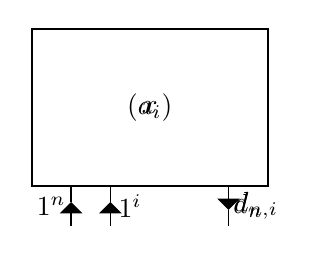
\begin{tikzpicture}<2->
				\path (0,0) rectangle (3.5,-2.7);
			%x
				\draw<2->[thick] (0,0) rectangle (3,-2);
				\node<2-3> at (1.5,-1) {$x$};
				\draw<2-> (.5,-2) -- (.5,-2.2);
				\draw<2->[-triangle 90] (.5,-2.5) -- (.5,-2.2);
				\node<2-> at (.25,-2.25) {$1^n$};
				\draw<2->[-triangle 90] (2.5,-2) -- (2.5,-2.3);
				\draw<2-> (2.5,-2.3) -- (2.5,-2.5);
				\node<2-3> at (2.75,-2.25) {$d_n$};
				\node<4-> at (2.85,-2.25) {$d_{n,i}$};
				\node<4-> at (1.5,-1) {$(a_i)$};
				\draw<4-> (1,-2) -- (1,-2.2);
				\draw<4->[-triangle 90] (1,-2.5) -- (1,-2.2);
				\node<4-> at (1.25,-2.25) {$1^i$};
		\end{tikzpicture}
		\end{figure}
		\begin{itemize}
			\item<3-> polynomial time computability
		\end{itemize}
	\end{minipage}
	\hfill
	\begin{minipage}{.45\textwidth}
		\onslide<2->{$d_n$ rational approximations}
		\only<2-4>{\[ \left|d_{n} - x\right|\leq 2^{-n}. \]}
		\only<5->{\[ \left|d_{n,i} - a_i\right|\leq 2^{-n}. \]}
	\end{minipage}
\end{frame}
\subsection{Real functions}

\begin{frame}
	\begin{minipage}{.45\textwidth}
		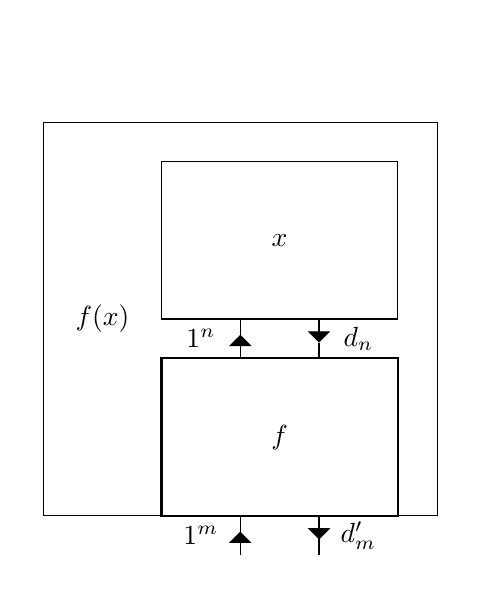
\begin{tikzpicture}
			\path (-1.7,1.7) rectangle (3.7,-5.2);
			%x
				\draw<2-> (0,0) rectangle (3,-2);
				\node<2-> at (1.5,-1) {$x$};
				\draw<1-> (1,-2) -- (1,-2.2);
				\draw<1->[-triangle 90] (1,-2.5) -- (1,-2.2);
				\node<2-> at (.5,-2.25) {$1^n$};
				\draw<1->[-triangle 90] (2,-2) -- (2,-2.3);
				\draw<1-> (2,-2.3) -- (2,-2.5);
				\node<2-> at (2.5,-2.25) {$d_n$};
			%f
				\draw<1->[thick] (0,-2.5) rectangle (3,-4.5);
				\node<1-> at (1.5,-3.5) {$f$};
				\draw<1-> (1,-4.5) -- (1,-4.7);
				\draw<1->[-triangle 90] (1,-5) -- (1,-4.7);
				\node<3-> at (.5,-4.75) {$1^m$};
				\draw<1->[-triangle 90] (2,-4.5) -- (2,-4.8);
				\draw<1-> (2,-4.8) -- (2,-5);
				\node<3-> at (2.5,-4.75) {$d'_m$};
			%f(x)
				\draw<3-> (-1.5,.5) rectangle (3.5,-4.5);
				\node<3-> at (-.75,-2) {$f(x)$};
		\end{tikzpicture}
	\end{minipage}
	\hfill
	\begin{minipage}{.47\textwidth}
		\begin{definition}
			\small
			A function $f:[0,1]\to\RR$ is called computable, \newline if there is a machine that,\newline when given oracle access to approximations to the argument $x$,\newline returns approximations to the value $f(x)$.
		\end{definition}
		\begin{itemize}
			\item<4-> Multivariate functions have more oracles.
			\item<5-> Computable functions are continuous.
		\end{itemize}
	\end{minipage}
\end{frame}
\subsection{iRRAM}
\begin{frame}[<+->]
\frametitle{iRRAM}
\begin{itemize}[<+->]
\item iRRAM is a C++ framework for exact real computations
\item Ordinary C++ is extended by datatype REAL for computing with real numbers
\item Usual arithmetic operations are implemented for REAL
\item Other functions like abs, power, root, modulo, exp, log, sin, cos are also available
\end{itemize}
\end{frame}
\begin{frame}[<+->][fragile]
\frametitle{Example: \irram}
\begin{example}
\begin{lstlisting}
REAL series(int n){
  return power(REAL(2), -n);
}
REAL xinv_approx(long p, REAL& x){
  int N=-2*p+3;
  REAL ans = 0.0;
  for(int i=0; i<=N; i++)
    ans += series(i)*power(x,i);
  return ans;
}
REAL xinv(REAL& x) { return limit(xinv_approx, x);}
\end{lstlisting}
\end{example}
\end{frame}

\begin{frame}
	\begin{beamercolorbox}[sep=8pt,center,shadow=true,rounded=true]{title}
      \usebeamerfont{title}
	Case Study: A Data Type for Analytic Functions\par%
    \end{beamercolorbox}
\vfill
\end{frame}
\section{Motivation}
\subsection{Analytic Functions}
\begin{frame}
\frametitle{Analytic Functions and Computational Complexity}
\begin{fact}
For general polynomial time computable functions, many important operators have been shown to be computationally hard.\\
For example
\begin{itemize}[<+->]
\item Polynomial time computable functions may have noncomputable derivatives. (Ko 1983)
\item Parametric maximization is NP-hard. (Ko/Friedman (1982))
\item Integration is \#P-hard. (Friedman (1984))
\end{itemize}
\end{fact}
\pause
We want to find a subset of polynomial time computable functions on which we can perform those operations in polynomial time.
\end{frame}
\begin{frame}
\frametitle{Analytic Function}
An analytic function is a function locally given by a complex power series.\\
\begin{definition}[Analytic Function]
% \begin{columns}
% \begin{column}{0.4\linewidth}
$f : D \to \C $, $D \subseteq \C$ is analytic if for any $x_0 \in D$ the Taylor-series
$$ T(x) := \sum^\infty_{n=0} a_n(x-x_0)^n$$
converges to $f(x)$ for $x$ in a neighborhood of $x_0$.  
% \end{column}
% \begin{column}{0.4\linewidth}
% \includegraphics[width=4.5cm]{TaylorComplexConv}
% \end{column}
% \end{columns}
\end{definition}
\end{frame}
\begin{frame}
\frametitle{Some non-uniform results}

$$a_m =\frac{f^{(m)}(x_0)}{m!} 
, \,\, f(x) = \sum_{m=0}^\infty a_m(x-x_0)^k \,\ \text{ for } x \in B(x_0,R)
$$
\vfill
\begin{theorem}[Pour-El, Richards, Ko, Friedman, M\"uller (1987/1989)]
$f$ is (polytime) computable iff $(a_m)_{m \in \N}$ is.
\end{theorem}
 \onslide<2->{
From that polynomial time computability of the derivative and the anti-derivative of a function follows immediately.
}
\end{frame}
\begin{frame}
\frametitle{Some non-uniform results}
$$a_m =\frac{f^{(m)}(0)}{m!} 
, \,\, f(x) = \sum_{m=0}^\infty a_mx^k \,\ \text{ for } x \in B(0,R)
$$
\vfill
\begin{theorem}[M\"uller (1995)]
\begin{itemize}
\item The operator $f \to (a_m)_{m \in \N}$ is not computable.
\item The evaluation operator $((a_m)_{m \in \N},x) \to f(x) $ is not computable.
\end{itemize}
\end{theorem}
\pause
However, if we supply some additional (discrete) information those operators become computable.
\end{frame}


\section{Representing power series}
\subsection{On the unit disc}
\begin{frame}
\frametitle{A practical representation for power series}
\begin{lemma}
Let $f : \C \to \C$ be analytic on the closed unit disc and $(a_m)_{m\in\N}$ its Taylor series around $0$.\\
Then $R>1$ \pause and we can find two positive integers $k$ and $A$ with 
\begin{itemize}
\item $r := \sqrt[k]{2}$ is strictly smaller than the radius of convergence $R$.
\item $|a_m|r^m \leq A$ for all $m \in \N$.
\end{itemize}
\end{lemma}
\pause
With $k$ and $A$ we can estimate 
$$ \left | \sum_{n \geq N} a_m z^n \right | \leq A\frac{(|z|/r)^N}{1-|z|/r} $$\pause
Consider triples $\big((a_m)_{n \in \N}, k, A\big)$ as representation for functions analytic on the unit disc.
\end{frame}
%\begin{frame}
%\frametitle{Finding $k$ and $A$}
%\begin{itemize}
%\item Choose $k$ appropriately and let $r := \sqrt{k}{2}$
%\item $f_{|z|=r}$ is a continuous function on a compact domain, thus is bounded by some number $A$
%\item By Cauchy Differentiation formula $$|a_n| \leq |\frac{1}{2\pi i}\int_{z=|r|} \frac{f(z)}{|z|^{n+1}} d \lambda| \leq \frac{A}{r^n}$$
%\end{itemize}
%\end{frame}
\begin{frame}[<+->]
\frametitle{Analytic Functions and Computational Complexity}
\begin{theorem}[Kawamura, R\"osnick, M\"uller, Ziegler (2013)]
  The following operators are computable in time polynomial in $k+log(A)+n$, where $2^{-n}$ is the output precision.
\begin{enumerate}
\item evaluation
\item addition and multiplication
\item differentiation and anti-differentiation
\item parametric maximization
\end{enumerate}
\end{theorem}
\end{frame}
\begin{frame}
\frametitle{But...}
\begin{center}
\includegraphics[width=0.6\textwidth]{TaylorComplexConv}
\end{center}
\end{frame}
\subsection{on $[-1,1]$}
\begin{frame}
\frametitle{\small Analytic functions on $[-1,1]$ (Kawamura, R\"osnick, M\"uller, Ziegler (2013))}
We want to consider complex functions analytic on $[-1,1]$.\\ 
\begin{minipage}{0.45\textwidth}
\begin{center}
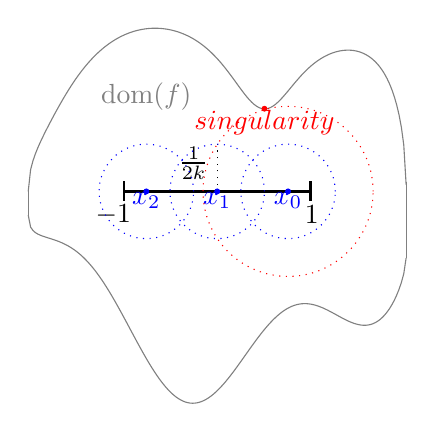
\begin{tikzpicture}[scale=0.6]
%    \draw<3> (-1,1) rectangle (5,-1);
    \node<1->  at (-0.2,-0.5) {$-1$};
    \node<1->  at (4.0,-0.5) {$1$};
    \draw<1-> [thick,|-|] (0,0) -- (4,0);
    \node<2>  at (1.5,.6) {$\frac 1{2k}$};
    \draw<2>  [dotted] (2.0,0) -- (2.0,1);
%    \node<3>  at (-.7,-.25) {$\frac 1l$};
%    \draw<3>  [dotted] (-1,0) -- (0,0);
%    \node<3>  at (2.2,.5) {$\frac 1l$};
%    \draw<3>  [dotted] (2,1) -- (2,0);
%    \node<3>  at (-.5,0.6) {$\overline R_l$};
    \draw<1-> [domain = 0:8,color=gray] plot[samples=160] (\x-2, {sqrt(16-(\x-4)^2)*(1-1/(\x^2+1) + sin(\x) + (\x/7)^5-\x/6 +1.5- 1/((\x-5)^2+1))/2});
    \draw<1-> [domain = 0:8,color=gray] plot[samples=160] (\x-2, {1/(\x^2+1)/2 + sin(80*\x) + (\x/7)^5-\x/6 -1-sqrt(16-(\x-4)^2)/2});
    \draw<1-> [color=gray] (-2,0) -- (-2,-.5);
    \draw<1-> [color=gray] (6,.19) -- (6,-1.42);
    \node<1-> [color=gray] at (.5,2) {$\dom(f)$};
    \draw<2> [fill=blue,radius =.05,color=blue] (3.5,0) circle;
    \node<2> [color=blue] at (3.5,-.2) {$x_0$};
    \draw<2> [fill=blue,radius =.05,color=blue] (2.0,0) circle;
    \node<2> [color=blue] at (2.0,-.2) {$x_1$};
    \draw<2> [radius = 1,color=blue, dotted] (2.0,0) circle; 
    \draw<2> [fill=blue,radius =.05,color=blue] (0.5,0) circle;
    \node<2> [color=blue] at (0.5,-.2) {$x_2$}; 
    \draw<2> [radius = 1,color=blue, dotted] (0.5,0) circle;
    \draw<2> [radius = 1,color=blue, dotted] (3.5,0) circle;
    \draw<2> [radius = 1.8, color = red, dotted] (3.5,0) circle; 
    \draw<1-> [fill=red,radius = .05,color = red] (3,1.75) circle;
    \node<1-> [color=red] at (3,1.45) {$singularity$};
    %\draw<3> [radius = 1, color = green, dotted] (2.5,0) circle;
    %\draw<3> [fill=green, radius = .05, color = green] (2.5,0) circle;
    %\node<3> [color=green] at (2.5,-.2) {$x_1$};
\end{tikzpicture}
\end{center}
\end{minipage}
\hfill
\begin{minipage}{0.45\textwidth}
\onslide<2->{
\begin{representation1}
  A finite number of taylor series together with parameters $A$ and $k$ that hold for each series, such that they cover the domain. 
 \end{representation1}
}
% \onslide<3->{
%\begin{representation2}
%A tuple $\big(f|_{[-1,1]}, B, l\big)$, $f \in C^\omega(\overline R_l)$ and $|f|_{\overline R_l}| \leq B$ where $\overline R_l := [-1-\frac1l,1+\frac1l]x[-\frac1l, \frac1l]$  
%\end{representation2}
%}
\end{minipage}
\end{frame}
%\begin{frame}
%\begin{minipage}{0.45\textwidth}
%\begin{representation1}
%A tuple $(M, (x_m), (a_{m,j}), A,k)$ $1 \leq m \leq M$, $j \in \N$ s.t. % with $1 \leq m \leq M$, $j \in \N$ so that
%%\item $a_{m,j}$ describes a Taylor series for $f$ around $x_m$ 
%$[-1,1] \subseteq \bigcup [x_m-\frac{1}{4k}, x_m+\frac{1}{4k}]$ \\
%and $|a_{m,j}| \leq A \cdot k^j$
% \end{representation1}
% \end{minipage}
% \hfill
% \begin{minipage}{0.45\textwidth}
%\begin{representation2}
%A tuple $\big(f|_{[-1,1]}, B, l\big)$, $f \in C^\omega(\overline R_l)$ and $|f|_{\overline R_l}| \leq B$ where $\overline R_l := [-1-\frac1l,1+\frac1l]x[-\frac1l, \frac1l]$  
%\end{representation2}
%\end{minipage}
%\begin{theorem}[Kawamura, R\"osnick, M\"uller, Ziegler (2013)]
%\begin{itemize}[<+->]
%\item Given $(M, (x_m), (a_{m,j}), A,k)$ we can evaluate $f(x)$ in time polynomial in $n+k+\lb(A)$
%\item From $(f,B,l)$ we can compute $(f^{(j)}(x_0))_{j \in \N}$ in time polynomial in $n+\lb(l)+\lb(B)$ 
%%and for all $x \in [-1,1]$ $|f^{(j)}(x)| \leq B\cdot l^j \cdot j!$
%\end{itemize}
%\end{theorem}
%\pause
%This means we can convert between those two representations in (parametrized) polynomial time.
%\end{frame} 

%\begin{frame}[<+->]
%\frametitle{Computing Taylor series}
%\begin{itemize}
%\item To convert between those representations we have to compute the Taylor coefficients from a given function
%\item Described in detail in (M\"uller87)
%\item Want to approximate the coefficient $a_m$ with max. error $2^{-n}$
%\item Approximate $f$ by Lagrangian interpolating polynomial $P_m(x) := \sum_{i=0}^{2m} f(x_i) \cdot L_{m,i}(x)$ with $L_{m,i}(x) = \prod_{j \neq i} \frac{x-x_j}{x_i-x_j} $ and $x_i = (i-m)\cdot h$
%\item Differentiate this polynomial $P^{(m)}(0) = \sum_{i=0}^{2m} f(z_i)\cdot L_{m,i}^{(m)}(0)$
%\item $\frac{1}{m!}P^{(m)}(0) = \sum_{i=0}^{2m} f(x_i)\frac{h^{-m}\cdot l_{m,i}}{i!(2m-i)!}$ with integers $l_{m,i}$
%\item An error bound for this approximation can be computed
%\end{itemize}
%\end{frame}


\begin{frame}
\frametitle{Evaluation}
\begin{minipage}{0.45\textwidth}

\begin{representation1}
  A finite number of taylor series together with parameters $A$ and $k$ that hold for each series covering the domain.
 \end{representation1}


\begin{representation2}
  A \textbf{single} taylor series together with parameters $A$ and $k$ that are valid for the the taylor series around any point of the domain.
\end{representation2}
\end{minipage}
\hfill
\begin{minipage}{0.45\textwidth}
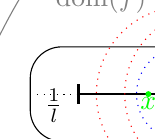
\begin{tikzpicture}[scale=0.6]
    \path [use as bounding box,red] (-30pt,-10pt) rectangle (30pt,40pt);
    \draw[rounded corners=4mm] (-1,1) rectangle (5,-1);
    %\draw (2,0) ellipse (3cm and 1cm);
    \draw [thick,|-|] (0,0) -- (4,0);
    \node at (-.5,-.25) {$\frac 1l$};
    \draw [dotted] (-1,0) -- (0,0);
    \node at (2.2,.5) {$\frac 1l$};
    \draw [dotted] (2,1) -- (2,0);
    \draw [domain = 0:8,color=gray] plot[samples=160] (\x-2, {sqrt(16-(\x-4)^2)*(1-1/(\x^2+1) + sin(\x) + (\x/7)^5-\x/6 +1.5- 1/((\x-5)^2+1))/2});
    \draw [domain = 0:8,color=gray] plot[samples=160] (\x-2, {1/(\x^2+1)/2 + sin(80*\x) + (\x/7)^5-\x/6 -1-sqrt(16-(\x-4)^2)/2});
    \draw [color=gray] (-2,0) -- (-2,-.5);
    \draw [color=gray] (6,.19) -- (6,-1.42);
    \node [color=gray] at (.5,2) {$\dom(f)$};
    \draw<1-3> [fill=blue,radius =.05,color=blue] (3.5,0) circle;
    \node<1-3> [color=blue] at (3.5,-.2) {$x_0$};
    \draw<1-3> [radius = 1,color=blue, dotted] (3.5,0) circle;
    \draw<1-3> [radius = 1.8, color = red, dotted] (3.5,0) circle; 
    \node<2> [color=red] at (2.5,-5) {Check if $x$ in circle};
    \draw [fill=green, radius = .05, color = green] (1.5,0) circle;
    \node [color=green] at (1.5,-.2) {$x$};
    \node<3> [color=red] at (3.0,-5) {Compute Taylor coefficients around $x_1$};
    \draw<3-5> [fill=cyan, radius = .05, color = cyan] (2.75,0) circle;
    \node<3-5> [color=cyan] at (2.75,-.2) {$x_1$};
    \draw<3-5> [radius = 1,color=cyan, dotted] (2.75,0) circle;
    \draw<4-5> [radius = 1.75, color = red, dotted] (2.75,0) circle; 
    \node<4> [color=red] at (2.5,-5) {Check if $x$ in circle};
    \node<5> [color=red] at (3.0,-5) {Compute Taylor coefficients around $x_2$};
    \draw<5-6> [fill=blue, radius = .05, color = blue] (2.25,0) circle;
    \node<5-6> [color=blue] at (2.25,-.2) {$x_2$};
    \draw<5-6> [radius = 1,color=blue, dotted] (2.25,0) circle;
    \draw<6> [radius = 1.85, color = red, dotted] (2.25,0) circle; 
\end{tikzpicture}
\end{minipage}
\end{frame}


\subsection{Implementation}
\begin{frame}[<+->]
\frametitle{Implementation}
\begin{itemize}
    \item A data type for functions real analytic on $[0,1]$ was implemented in \irram .
    \item Constructor from a single power series.
    \item Analytic continuation used if more series are needed to cover the interval. 
    \item The running time and memory usage was empirically analyzed.
    \item Running time increases quickly with number of analytic continuations. 
\end{itemize}
\end{frame}
\begin{frame}[t]{Riemann Mapping Theorem}
  \begin{theorem}[Riemann]
    Let $U \subsetneq \C$ be non empty, simply connected and open.\\
    Then there exists a biholomorphic mapping from $U$ on to the open unit disc.
%\begin{tikzpicture}[scale=0.9]
%    \path [use as bounding box,red] (-100pt,-10pt) rectangle (30pt,40pt);
%    \draw (-3,0.5) rectangle (2,-0.5);
%    \draw [thick,->] (2.2,0) -- (3.8,0);
%    \draw (5,0) ellipse (1cm and 1cm);
%\end{tikzpicture}
  \end{theorem}
\vfill \pause
 How complex is it to compute this mapping?\\
  \pause
  In the general case $\#P$ hard (Binder, Braverman, Yampolsky).\\
  \pause
  Riemann mappings of domains with polynomial time computable analytic boundaries are polynomial time computable (Rettinger).
\end{frame}
\begin{frame}[<+->]{Summary}
 When developing Exact Real Arithmetic algorithms the following is important
 \begin{itemize}
     \item Careful mathematical analysis of the errors that arise by finite approximations has to be performed.
     \item Theorems from real and complex analysis have to be combined with methods from theoretical computer science to get efficient algorithms.
     \item Finding the right restriction of the type of functions considered, so that efficient algorithms are possible but the class still contains most functions relevant in practice.
     \item It is sometimes necessary to enrich the input by natural parameters of the function to gain better computability or complexity results.
 \end{itemize}
\end{frame}

\begin{frame}
	\begin{beamercolorbox}[sep=8pt,center,shadow=true,rounded=true]{title}
      \usebeamerfont{title}
	Case Study: Dynamic Systems and the Shadowing Lemma\par%
    \end{beamercolorbox}
\vfill
\end{frame}
\section{Dynamic Systems and the Shadowing Lemma}
\subsection{Overview}
\begin{frame}[<+->]
\frametitle{Shadowing}
Consider the logistic map $f(x) = a x  (1-x)$ for $a \in \RR$ \\
The orbit of $f$ is given by the recurrence 
$y_{i+1} = f(y_i)$ and $y_0 \in \RR$.
\pause
\begin{definition}
	The sequence $(x_i)$ is called an $\alpha$-pseudo-orbit for $f$ if 
	$$
	\| x_{i+1} - f(x_i) \| < \alpha
	$$ 
	A real orbit $(y_i)$ $\beta$-shadows a pseudo-orbit $(x_i)$ if 
	$$
	\| x_{i} - y_i \| < \beta
	$$ 
\end{definition}
\pause
Question (originally considered by Hammel, Yorke and Grebogi in 1987): How long does a shadowing orbit for the logistic map exist for different parameters $a$ and $x_0$?
\end{frame}
\begin{frame}[<+->]
\frametitle{Computing the shadowing orbit}
\begin{itemize}
\item \irram can be used to exactly compute a shadowing orbit of length $N$
\item First compute the psuedo orbit $(x_i)$
\item Start with $y_N := x_N$ and iteratively compute $y_{i-1} = f^{-1}(y_i)$
\item For $f^{-1} = 0.5 \pm \sqrt{0.25-\frac{x}{a}}$ choose the value that is on the same side of $0.5$ as $x_i$
\item The backward procedure will stay close to the pseudo-orbit since $f^{-1}$ is a contraction.
\item Note that the algorithm might fail
\end{itemize}
\end{frame}
\begin{frame}
	\begin{beamercolorbox}[sep=8pt,center,shadow=true,rounded=true]{title}
      \usebeamerfont{title}
	Future Work\par%
    \end{beamercolorbox}
\vfill
\end{frame}
\subsection*{Future}
\begin{frame}[<+->]
  \frametitle{Future Work}
\begin{itemize}
    \item Extend class for analytic functions to multi dimensional case
    \item Solver for ODEs with analytic right hand sides
    \item Detailed Analysis of Numerical ODE solvers
	\item Parametrized analysis of such approaches will be performed
	\item taking into account the number of steps and the intermediate precision required to attain guaranteed
output error $2^{-n}$
\end{itemize}
\end{frame}

\begin{frame}

    \vspace{\fill}
\begin{beamercolorbox}[center,shadow=true,rounded=true]{note} 
        \huge Thank you!
\end{beamercolorbox}

    \vspace{\fill}
\end{frame} 
{
\makeatletter % to change template
    \setbeamertemplate{headline}[default] 
    \def\beamer@entrycode{\vspace*{-\headheight}} 
\makeatother
\begin{frame}{References}
\fontsize{6pt}{7.2}\selectfont 
\nocite{*}
\def\newblock{}
\bibliographystyle{abbrv}

\begin{thebibliography}{10}   

  \beamertemplatearticlebibitems
  \bibitem{6}
	Harvey Friedman,
    \newblock \emph{ The computational complexity of maximization and integration}, Adv. in Math. 53 (1984), no. 1, 80-98. MR 748898 (86c:03037)
  \beamertemplatearticlebibitems
  \bibitem{1}
	Akitoshi Kawamura, Norbert Th. M\"{u}ller, Carsten R\"{o}snick, and
Martin Ziegler
    \newblock \emph{Parameterized Uniform Complexity in Numerics:
from Smooth to Analytic, from NP-hard to Polytime}, pre-print (2012).

  \beamertemplatearticlebibitems
  \bibitem{7}
	Ker-I Ko,
    \newblock \emph{ Complexity theory of real functions}, Progress in Theoretical Computer Science, Birkh\"{a}user Boston Inc., Boston, MA, 1991.
MR 1137517 (93i:03057)

  \beamertemplatearticlebibitems
  \bibitem{8}
	Ker-I Ko,
    \newblock \emph{  On the Computational Complexity of Ordinary Differential Equations}, Information and Control 58(1-3): 157-194 (1983)


  \beamertemplatearticlebibitems
  \bibitem{2}
	Norbert Th. M\"{u}ller,
    \newblock \emph{ The \irram: Exact Real Arithmetic in C++}, Computability and Complexity in Analysis (2000) .

  \beamertemplatearticlebibitems
  \bibitem{Mul95}
	Norbert Th. M\"{u}ller,
    \newblock \emph{ Constructive aspects of analytic functions}, Computability
and Complexity in Analysis (Ker-I Ko and Klaus Weihrauch, eds.),
Informatik Berichte, vol. 190, FernUniversit\"{a}t Hagen, September
1995, CCA Workshop, Hagen, August 19-20, 1995, pp. 105-114.

  \beamertemplatearticlebibitems
  \bibitem{4}
	Norbert Th. M\"{u}ller,
    \newblock \emph{ Uniform Computational Complexity of Taylor Series}, ICALP 1987: 435-444

  \beamertemplatearticlebibitems
  \bibitem{5}
	Norbert Th. M\"{u}ller,
    \newblock \emph{ Polynomial Time Computation of Taylor Series}, Proc. 22 JAIIO - PANEL 1993

  \beamertemplatearticlebibitems
  \bibitem{9}
	Marian B. Pour-El and J. Ian Richards,
    \newblock \emph{ Computability in analysis
and physics}, Perspectives in Mathematical Logic, Springer-Verlag,
Berlin, 1989. MR 1005942 (90k:03062)
  \beamertemplatearticlebibitems
  \bibitem{11}
	Florian Steinberg,
    \newblock \emph{A type of Taylor series for the C++ library iRRAM for exact real arithmetic} (draft) last edited November 28, 2013
  \beamertemplatearticlebibitems
  \bibitem{10}
	Klaus Weihrauch,
    \newblock \emph{Computable analysis}, Texts in Theoretical Computer
Science. An EATCS Series, Springer-Verlag, Berlin, 2000, An
introduction. MR 1795407 (2002b:03129)

  \end{thebibliography}

\end{frame}
}
\end{document}
